\documentclass[aspectratio=169]{beamer}
% \setbeamertemplate{footline}[frame number]
\usepackage{color,amsmath}
\usepackage{subfigure}
\usepackage{booktabs}
\usepackage{framed}
\usepackage{comment}
\hypersetup{
colorlinks=true,
linkcolor=blue,
filecolor=magenta,      
urlcolor=blue,
pdftitle={Overleaf Example},
pdfpagemode=FullScreen}
\usepackage{tabularx}

%%%%%%%%%%%%%%%%%%%%%%%%%%
\title[]{Survey research in the digital age}
\author[]{Bernhard Clemm von Hohenberg\\Department of Computational Social Science\\GESIS}
\date[]{Summer Institutes in Computational Social Science\\July 28, 2023}
\begin{document}
%%%%%%%%%%%%%%%%%%%%%%%%%%
\frame{\titlepage}
%%%%%%%%%%%%%%%%%%%%%%%%%%

\begin{frame}{Schedule}

\vspace{0.5em}
\begin{itemize}
\item 9.00-9.45 Introduction \& total error survey framework
\item 9.45-10.15 Probability and non-probability sampling
\vspace{0.5em}
\item Coffee break
\vspace{0.5em}
\item 10.30-11.00 Computer-administered interviewing
\item 11.00-11.30 Linking surveys to big data
\item 11:30-13:00 Intro and begin group exercise
\vspace{0.5em}
\item Lunch (or Eisbach plunge)
\vspace{0.5em}
\item 14:00-15:45 Continue group exercise
\end{itemize}

\end{frame}
%%%%%%%%%%%%%%%%%%%%%%%%%%%
\begin{frame}{Credits}

These materials build heavily on Matthew Salganik's 2019 SICSS class as well as Chapter 3 of ``Bit by Bit: Social Research in the Digital Age''.

\end{frame}
%%%%%%%%%%%%%%%%%%%%%%%%%%%
\begin{frame}{Background readings}

\begin{itemize}
\item Salganik, Matthew J. \textit{Bit by bit: Social research in the digital age.} Princeton University Press, 2019. Chapter 3. 
\href{https://www.bitbybitbook.com/en/1st-ed/asking-questions}{Link}.
\item Berinsky, Adam J. ``Measuring public opinion with surveys.'' \textit{Annual Review of Political Science} 20 (2017): 309-329. \href{https://www.annualreviews.org/doi/abs/10.1146/annurev-polisci-101513-113724}{Link}.
\item Barabas, Jason and Jennifer Jerit. ``Are Nonprobability Surveys Fit for Purpose?'' Forthcoming in \textit{Public Opinion Quarterly}. \href{https://bpb-us-e1.wpmucdn.com/sites.dartmouth.edu/dist/d/2388/files/2023/05/JeritBarabas_NPS_Mar2023-1.pdf}{Link}.
\item Barabas, Jason and Jennifer Jerit. ``Are Nonprobability Surveys Fit for Purpose?'' Forthcoming in \textit{Public Opinion Quarterly}. \href{https://bpb-us-e1.wpmucdn.com/sites.dartmouth.edu/dist/d/2388/files/2023/05/JeritBarabas_NPS_Mar2023-1.pdf}{Link}.
\item Goel, Sharad, et al. ``Online, Opt-in Surveys: Fast and Cheap, but are they Accurate?''. \textit{Working Paper}, 2017. \href{https://5harad.com/papers/dirtysurveys.pdf}{Link}.

\end{itemize}

\end{frame}
%%%%%%%%%%%%%%%%%%%%%%%%%%%
\begin{frame}

\begin{center}
\LARGE{Why should I care about surveys\\in the age of big data?}
\end{center}

\end{frame}
%%%%%%%%%%%%%%%%%%%%%%%%%%%%%
\begin{frame}{Surveys and big data}

Digital age provides tons of data about people, e.g., 
\begin{itemize}
\item Online manifestations of attitudes and behaviors
\pause
\item Structure of social networks (literally speaking)
\pause
\item Digitized administrative data 
\end{itemize}

\end{frame}
%%%%%%%%%%%%%%%%%%%%%%%%%%%%%
\begin{frame}

\begin{center}
\LARGE{But what can I really learn from this?}
\vfill
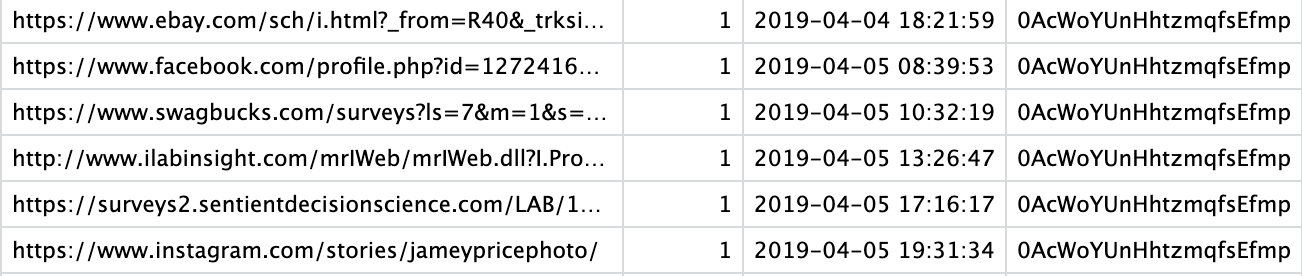
\includegraphics[width=0.9\textwidth]{figures/trace-data.png}
\end{center}

\end{frame}
%%%%%%%%%%%%%%%%%%%%%%%%%%%%%
\begin{frame}{Limits of big data}

We can learn some things from big data---but there are limits:
\begin{itemize}
\item Inaccuracy, inaccessibility and incompleteness
\pause
\item Internal states vs. external states
\pause
\begin{itemize}
\item Social desirability bias in the online sphere 
\pause
\item Measuring the ``subconscious'' from digital traces
\end{itemize}
\end{itemize}


\vfill

\end{frame}
%%%%%%%%%%%%%%%%%%%%%%%%%%%
\begin{frame}

\begin{center}
\LARGE{We will always need to ask---but how we ask will change.}
\end{center}

\end{frame}
%%%%%%%%%%%%%%%%%%%%%%%%%%%
\begin{frame}{Eras of survey research}

\begin{center}
\renewcommand{\arraystretch}{1.5}
\begin{tabular}{p{0.08\textwidth}p{0.26\textwidth}p{0.24\textwidth}p{0.24\textwidth}}
& \textbf{Sampling} & \textbf{Interviews} & \textbf{Data environment}\\
\hline
\hline
1st era & Area probability & Face-to-face & Stand-alone \\
\end{tabular}
\end{center}

\end{frame}
%%%%%%%%%%%%%%%%%%%%%%%%%%%
\begin{frame}{Eras of survey research}

\begin{center}
\renewcommand{\arraystretch}{1.5}
\begin{tabular}{p{0.1\textwidth}p{0.26\textwidth}p{0.24\textwidth}p{0.24\textwidth}}
& \textbf{Sampling} & \textbf{Interviews} & \textbf{Data environment}\\
\hline \hline
1st era & Area probability & Face-to-face & Stand-alone \\
\hline
2nd era & Random digital dial probability & Telephone & Stand-alone \\
\end{tabular}
\end{center}


\end{frame}
%%%%%%%%%%%%%%%%%%%%%%%%%%%
\begin{frame}{Eras of survey research}

\begin{center}
\renewcommand{\arraystretch}{1.5}
\begin{tabular}{p{0.1\textwidth}p{0.26\textwidth}p{0.24\textwidth}p{0.24\textwidth}}
& \textbf{Sampling} & \textbf{Interviews} & \textbf{Data environment}\\
\hline \hline
1st era & Area probability & Face-to-face & Stand-alone \\
\hline
2nd era & Random digital dial probability & Telephone & Stand-alone \\
\hline
3rd era & Non-probability & Computer-administered  & Linked \\
\end{tabular}
\end{center}

\end{frame}
%%%%%%%%%%%%%%%%%%%%%%%%%%%
\begin{frame}
\begin{center}
\renewcommand{\arraystretch}{1.5}
\begin{tabular}{p{0.1\textwidth}p{0.26\textwidth}p{0.24\textwidth}p{0.24\textwidth}}
& \textbf{Sampling} & \textbf{Interviews} & \textbf{Data environment}\\
\hline \hline
1st era & Area probability & Face-to-face & Stand-alone \\
\hline
2nd era & Random digital dial probability & Telephone & Stand-alone \\
\hline
\textcolor{violet}{3rd era} & \textcolor{violet}{Non-probability} & \textcolor{violet}{Computer-administered}  & \textcolor{violet}{Linked} \\
\end{tabular}
\end{center}

\end{frame}
%%%%%%%%%%%%%%%%%%%%%%%%%%%
\begin{frame}


\begin{center}
\LARGE{Total survey error framework}
\end{center}

\end{frame}
%%%%%%%%%%%%%%%%%%%%%%%%%%%
\begin{frame}{TSE framework}

Total survey error = representation error + measurement error
\pause
\vspace{1em}

\begin{columns}[T]

\begin{column}{0.45\textwidth}
Who we ask (representation)\\
\begin{itemize}
\item sampling error
\item coverage errors
\item non-response error
\end{itemize}
\end{column}
\pause
\begin{column}{0.45\textwidth}
How we ask (measurement)\\
\begin{itemize}
\item question wording
\item question ordering
\item social desirability bias
\item mode/device effects
\end{itemize}
\end{column}

\end{columns}

\end{frame}
%%%%%%%%%%%%%%%%%%%%%%%%%%%
\begin{frame}{TSE framework}

Total survey error = representation error + measurement error
\vspace{1em}

\begin{columns}[T]

\begin{column}{0.45\textwidth}
\textcolor{violet}{Who we ask (representation)}\\
\begin{itemize}
\item sampling error
\item coverage errors
\item non-response error
\end{itemize}
\end{column}

\begin{column}{0.45\textwidth}
How we ask (measurement)\\
\begin{itemize}
\item question wording
\item question ordering
\item social desirability bias
\item mode/device effects
\end{itemize}
\end{column}

\end{columns}

\end{frame}
%%%%%%%%%%%%%%%%%%%%%%%%%%%
\begin{frame}{TSE framework}

\begin{center}
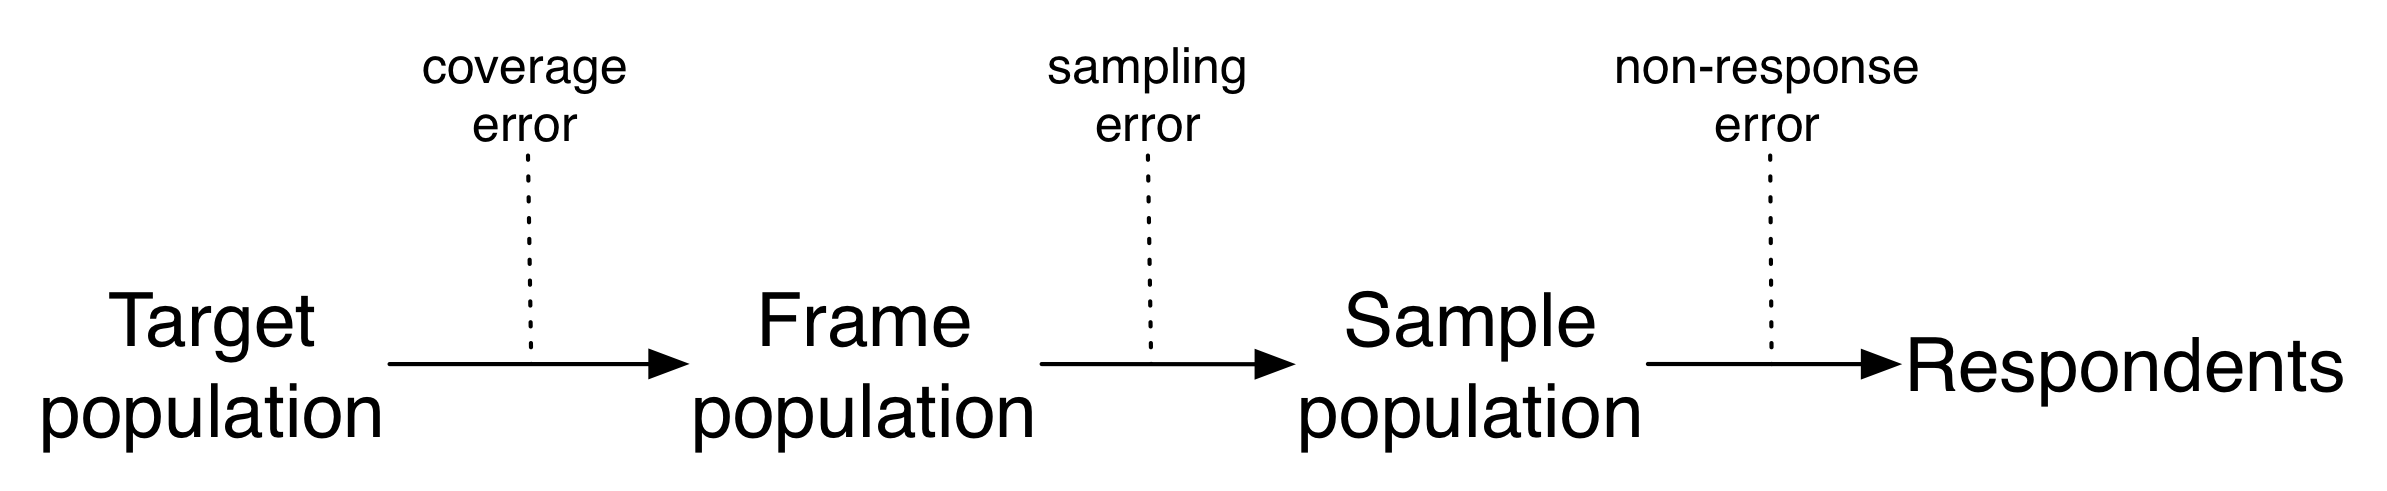
\includegraphics[width=\textwidth]{figures/bitbybit3-2_representation_errors.png}
\end{center}

\end{frame}
%%%%%%%%%%%%%%%%%%%%%%%%%%%
\begin{frame}{TSE framework}
\begin{center}
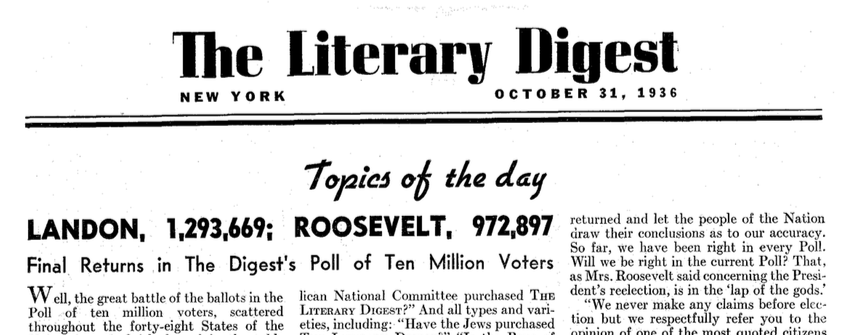
\includegraphics[width=0.9\textwidth]{figures/literary-digest.png}
\end{center}

\end{frame}
%%%%%%%%%%%%%%%%%%%%%%%%%%
\begin{frame}{TSE framework}

Total survey error = representation error + measurement error
\vspace{1em}

\begin{columns}[T]

\begin{column}{0.45\textwidth}
Who we ask (representation)\\
\begin{itemize}
\item sampling error
\item coverage errors
\item non-response error
\end{itemize}
\end{column}

\begin{column}{0.45\textwidth}
\textcolor{violet}{How we ask (measurement)}\\
\begin{itemize}
\item question wording
\item question ordering
\item social desirability bias
\item mode/device effects
\end{itemize}
\end{column}

\end{columns}

\end{frame}
%%%%%%%%%%%%%%%%%%%%%%%%%%%
\begin{frame}{TSE framework}

\begin{columns}[T]

\begin{column}{0.48\textwidth}
\begin{center}
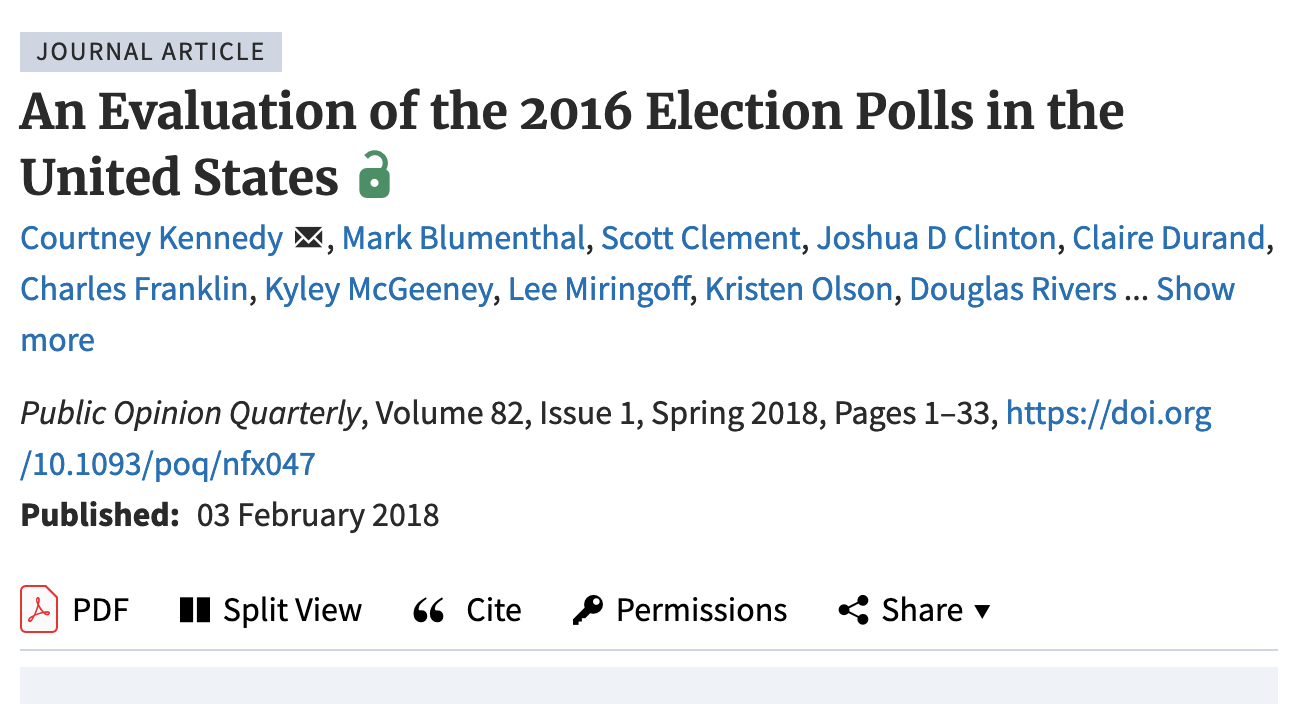
\includegraphics[width=\textwidth]{figures/aapor-2016.png}
\end{center}
\end{column}

\begin{column}{0.48\textwidth}
\vspace{1em}
``Some Trump voters who participated in pre-election polls did not reveal themselves as Trump voters until after the election, and they outnumbered late-revealing Clinton voters''  \\
\vspace{1em}
\TINY{\url{https://academic.oup.com/poq/article/82/1/1/4837043}}

\end{column}

\end{columns}



\end{frame}
%%%%%%%%%%%%%%%%%%%%%%%%%%%%%%
\begin{frame}{TSE framework}

In sum, total survey error framework...
\begin{itemize}
\item ... helps us organize all the things that can go wrong
\pause
\item ... also helps us think about how digital age can create new opportunities
\end{itemize}

\end{frame}
%%%%%%%%%%%%%%%%%%%%%%%%%%%%%%
\begin{frame}

\begin{center}
\Large Questions
\end{center}

\end{frame}
%%%%%%%%%%%%%%%%%%%%%%%%%%%%%%





\end{document}